\documentclass[12pt,letterpaper, onecolumn]{exam}
\usepackage{amsmath}
\usepackage{amssymb}
\usepackage{graphicx}
\usepackage[lmargin=71pt, tmargin=1.2in]{geometry}  %For centering solution box

% \chead{\hline} % Un-comment to draw line below header
\thispagestyle{empty}   %For removing header/footer from page 1

\begin{document}

\begingroup  
    \centering
    \LARGE STATS 212\\
    \LARGE Homework# 4 \\[0.5em]
    \large \today\\[0.5em]
    \large Samuel Molero\par
    \large samueljosemolero@tamu.edu\par
    \large Section: 501\par
\endgroup
\rule{\textwidth}{0.4pt}
\pointsdroppedatright   %Self-explanatory
\printanswers
\renewcommand{\solutiontitle}{\noindent\textbf{Ans:}\enspace}   %Replace "Ans:" with starting keyword in solution box

\begin{questions}
    \question Q1?
    \begin{solution}
        \begin{parts}
            \part 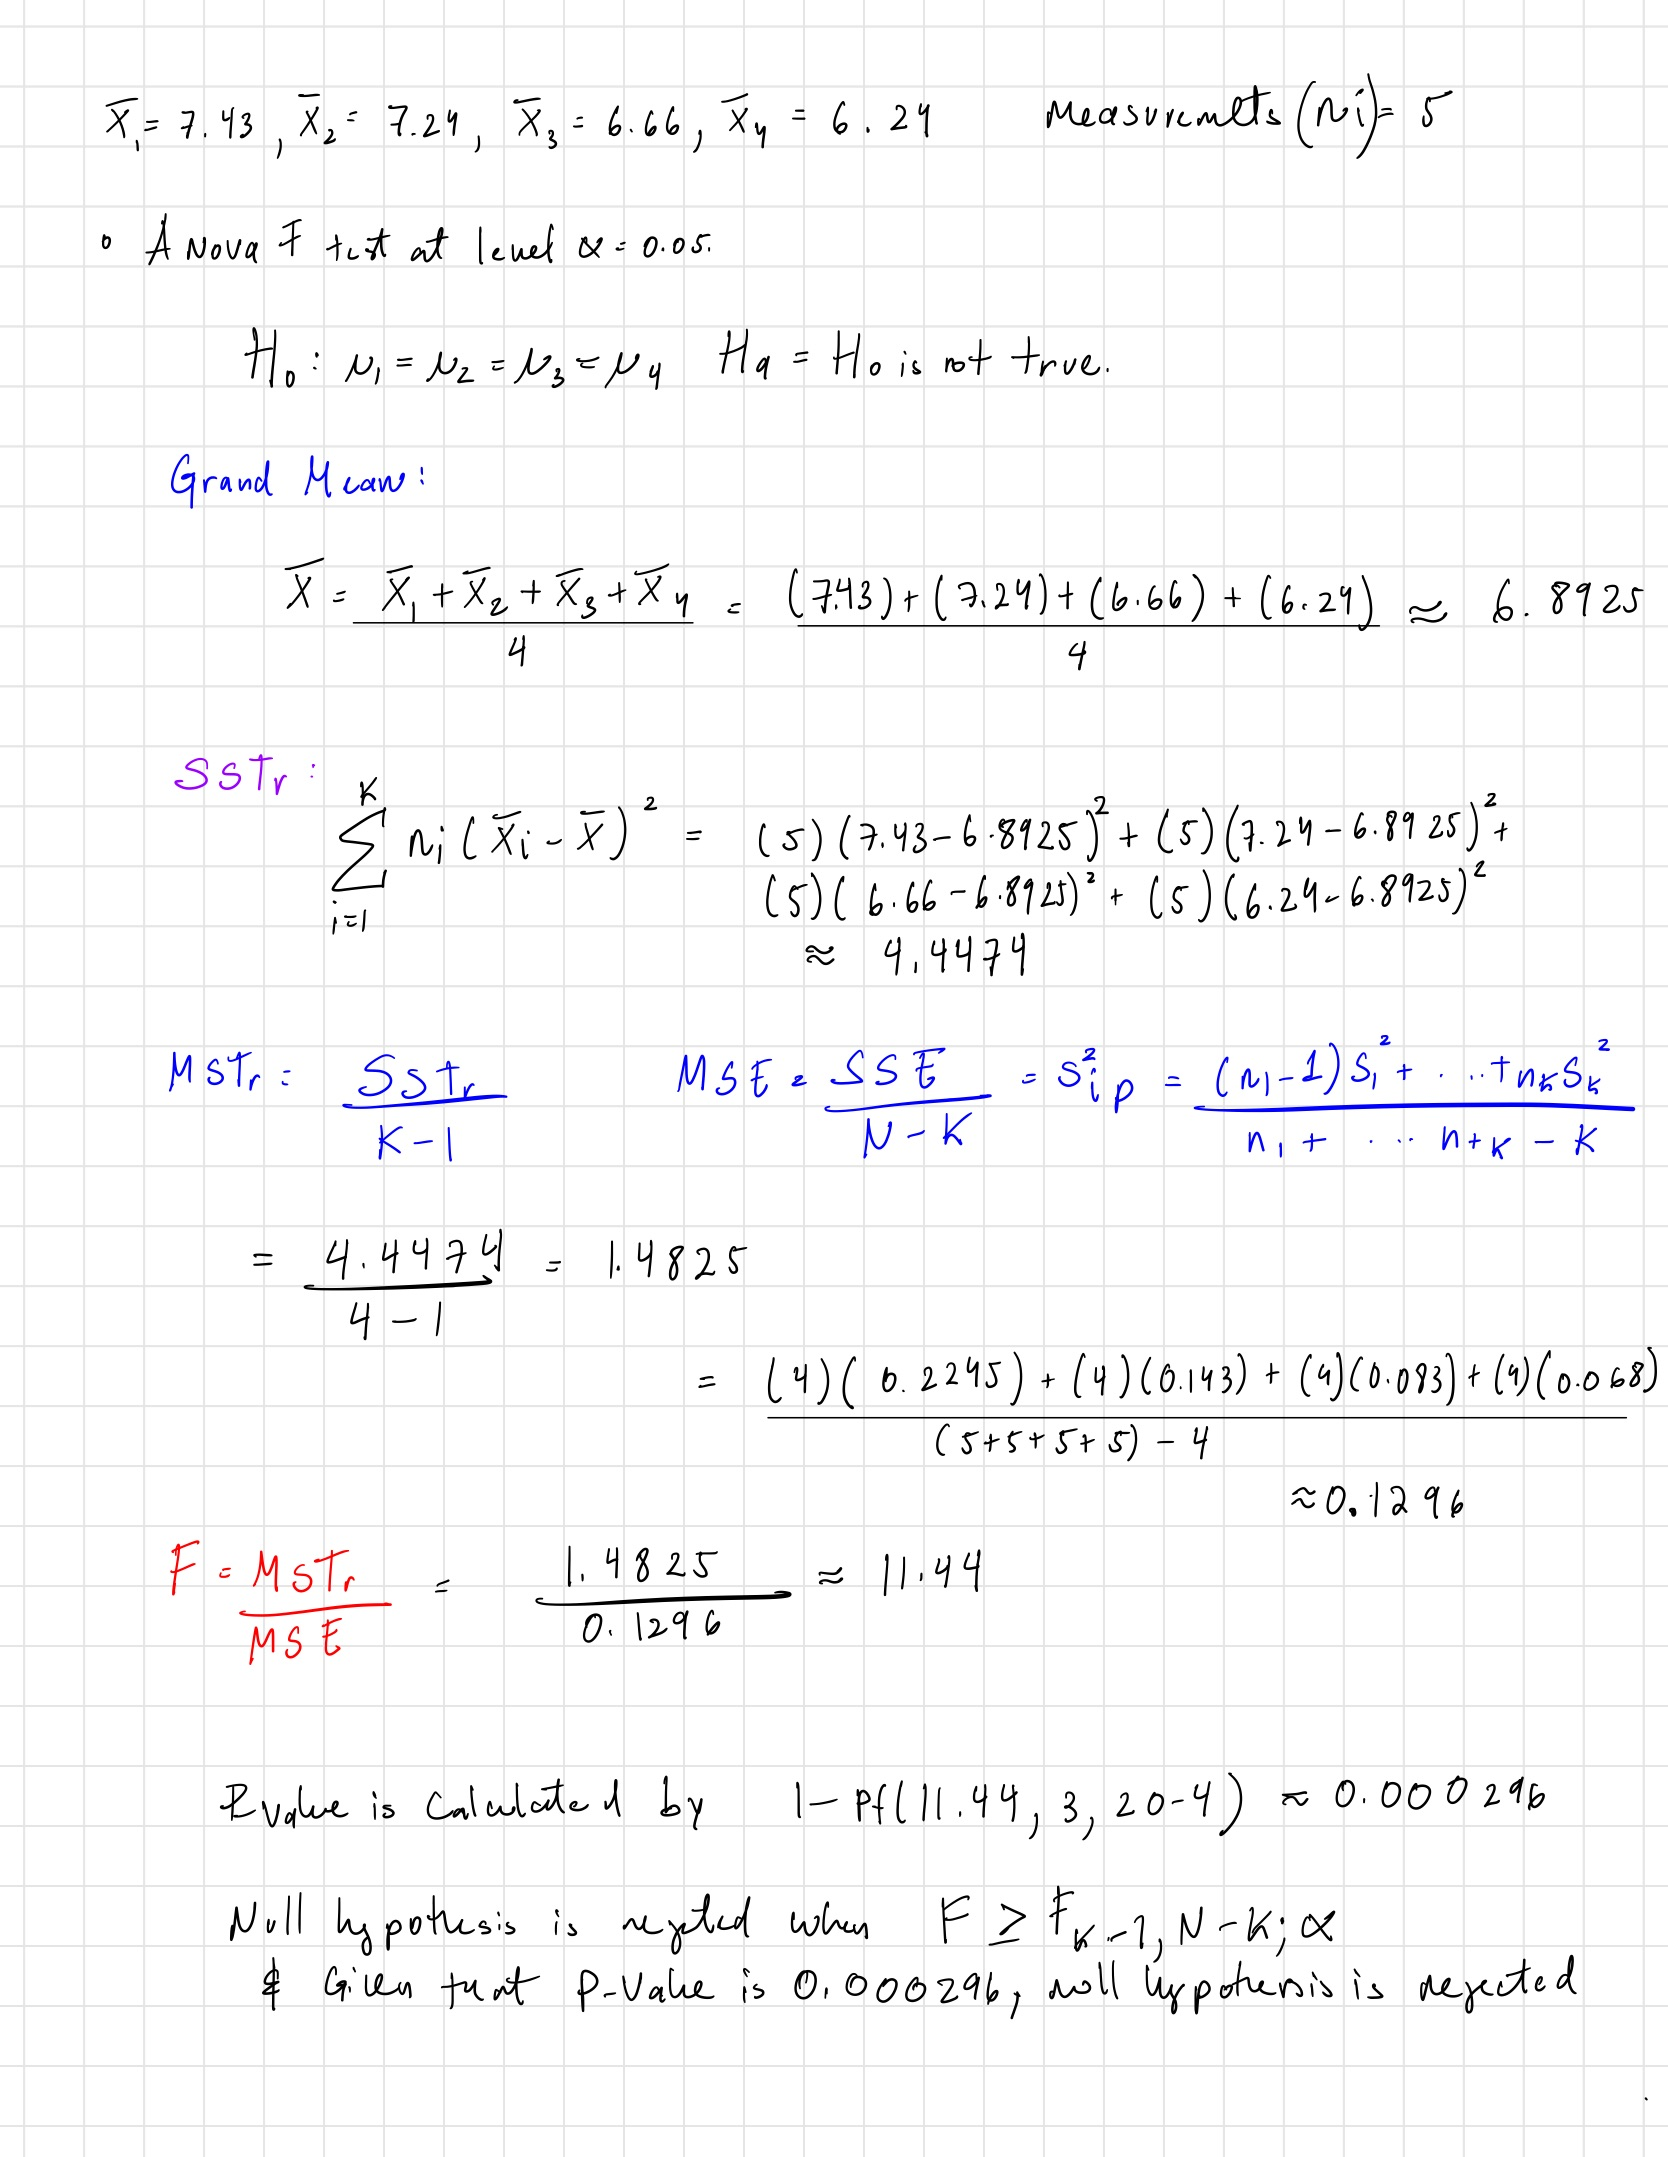
\includegraphics[width=0.70\textwidth]{Homeworks/Homework4A.jpg}
            \part 
    \begin{verbatim}
    pc_aov <- aov(values ~ as.factor(temp), data = pc)
    anova(pc_aov)
    \end{verbatim}

    Using the code above, the F-value is $11.437$ and the p-value is $0.0002958$.
    Rejecting the null at a significant level of 0.05, given that the p-value is smaller.

    \part
    \begin{verbatim}
        anova(aov(resid(aov(values ~ temp))**2 ~ temp)) (1)
        shapiro.test(resid(aov(values~temp))) (2)
        
        qqnorm(resids) (3)
        qqline(resids)
        boxplot(resids, main ="Boxplot of residuals") (4)
    \end{verbatim}

    Using the first code snippet to determine the assumption of equal variance returns a p-value of $0.0656$, demonstrating a valid assumption of equal variance. For normality, the second code snippet is used to return a p-value of $0.8255$, showing that the normality assumption holds.\\

    Using the third and fourth code Snippet will result in the following graphs respectively:

    
    

    
            
        \end{parts}
        
    \end{solution}
    
    
\end{questions}
\end{document}